
\section{MQTT Payload Encryption/Authentication }

In Chapter 6, payload encryption was discussed as a means of ensuring message confidentiality at the application level. This approach can be used to establish an end-to-end secure channel between the sender and receiver at the application level  to provide confidentiality over transmitted data. However, in this paper, we extend the scope beyond message confidentiality and introduce the ASCON algorithm to provide both message authenticity and confidentiality.

Furthermore, in this paper, we use the device id as associative or additional data used along the key and plain text as input for the implementation of the ASCON and AES-GCM algorithms. It is important to highlight that the device ID and its corresponding private key are assumed to be pre-shared between the communicating parties prior to initiating communication. In our case, while the device id is managed and maintained by the Digital Twin device registration module, the symmetric key should be explicitly configured from both side of the implementtion.  

The MQTT protocol is a lightweight messaging protocol that is often used in the Internet of Things (IoT). MQTT protocol can be configured and programmed to supports payload encryption using any encryption algorithm, including the ASCON and AES-GCM. 


\begin{figure}[H]
    \caption{Scheme of Payload Encryption With Authentication Over MQTT Protocol. }
    \centering
    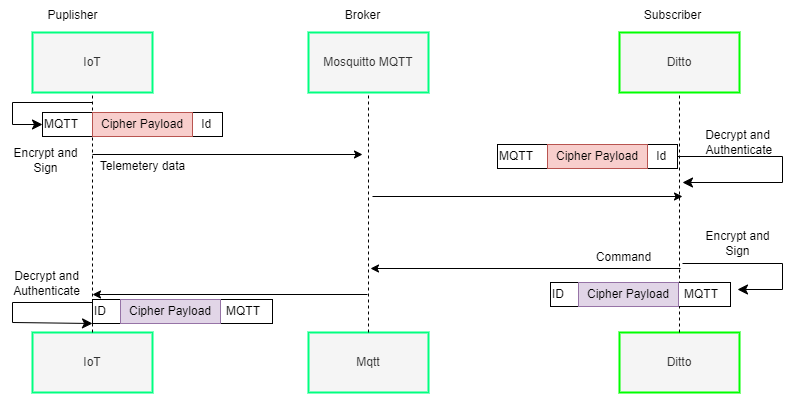
\includegraphics[width=\textwidth]{images/fp/payloadenc.drawio.png}
    \label{fig:payload-encauth-schem}
\end{figure}

To achieve payload encryption using ASCON or AES-GCM algorithm over the MQTT protocol, the following steps should be taken. 
\begin{itemize}
    \item[-] \textit{Device ID registration}: Each connected device to Ditto should have a unique device id. 
    \item[-] \textit{Generate and manage encryption keys}: The device and the Digital Twin agree on a symmetric key. 
    \item[-] \textit{Encryption and Sending a message}: The sender encrypts the payload of the message along with a tag generated and publishes it to the MQTT broker. In this case, associated data is the unique id of the device sending and receiving data to and from the Digital Twin. 
    \item[-] \textit{Forwarding or Proxing}: The MQTT broker proxies the message through the publisher-subscriber setting. 
    \item[-] \textit{Decryption and Authentication}: The receiver (subscriber) receives the MQTT message and decrypts and authenticates the payload using the agreed key and claimed device ID.
    
\end{itemize}


\subsection{End-To-End Encryption and Authentication}
Our communication scheme based on payload encryption and authentication using one of the AEAD (authenticated encryption with associated data) algorithms over the MQTT protocol implicitly provides end-to-end confedentiality and integrity of a communicated message. The Mosquitto broker acts as a proxy for forwarding encrypted payload messages, which are eventually decrypted and authenticated by the receiving application. 